%======================================================================
\section{Data and calibration}\label{sec:calibration}
%======================================================================

\subsection{Data}

\paragraph{Bond prices.} Daily Capital IQ evaluated bid, mid and ask prices for the three
AT1s, the two Tier~2 notes and the SNP note, from each bond's issue date (the earliest
being 27 June 2025) to 25 September 2026. Grey-market quotes before the issue date are
discarded, as are weekend repetitions of Friday's evaluation. The analysis uses weekly
(Friday) observations, 66 dates. Accrued interest is computed on a 30/360 basis on the
trade date and matches Capital IQ's ``T0 accrued interest'' to three decimals. Evaluated
prices are composites of dealer quotes rather than transactions; their bid--offer on the
valuation date is $0.15$--$0.29$ points for the AT1s and $0.07$--$0.17$ for the Tier~2 and
SNP notes, all of which carry Capital IQ's highest liquidity score.

\paragraph{Treasury curve.} FRED constant-maturity Treasury yields at five, seven and ten
years (DGS5, DGS7, DGS10). The five-year CMT is the reset reference of the AT1s; each bond is
discounted at the yield interpolated linearly at its time to first call, flat outside the
five-to-ten-year range.

\paragraph{Capital.} Quarterly CET1 ratios from Capital IQ, 2014Q1 to 2026Q2. Earlier data
follow Basel~II/2.5 definitions and are not comparable. A print is used only from 35 days
after the quarter end, approximating BNP's publication lag. The CET1 requirement is the
year-end stack from Capital IQ up to 2024 and the quarterly figures published by BNP
thereafter ($10.51\%$ at September 2025, $10.43\%$ at June 2026).

\paragraph{Credit default swaps.} BNP Paribas senior CDS, EUR, MM14 documentation:
the five-year conventional spread daily since October 2023 and full curves on six
snapshot dates. The CDS is used only as a reference point, because it is quoted in a
different currency and is referenced to senior rather than subordinated debt.

\paragraph{Other.} BNP's share price (EUR) and the EBA 2025 stress test results, in which
BNP's fully loaded CET1 ratio falls by $4.21$pp in the adverse scenario.

\subsection{Capital dynamics}

\paragraph{Likelihood.} Ignoring jumps, the CET1 process is an Ornstein--Uhlenbeck process
whose transition over a step $\Delta_k$ is Gaussian:
\begin{equation}\label{eq:outrans}
  C_{k+1}\mid C_k\sim N\bigl(m_k,\ \sigma^2w_k\bigr),\qquad
  m_k=\theta+(C_k-\theta)e^{-\kappa\Delta_k},\qquad
  w_k=\frac{1-e^{-2\kappa\Delta_k}}{2\kappa}.
\end{equation}
The exact log-likelihood of $n$ transitions is
\begin{equation}\label{eq:loglik}
  \ell(\kappa,\sigma)=-\frac12\sum_{k}\Bigl[\log\bigl(2\pi\sigma^2w_k\bigr)
  +\frac{(C_{k+1}-m_k)^2}{\sigma^2w_k}\Bigr].
\end{equation}
For fixed $\kappa$ the maximiser in $\sigma$ is available in closed form,
\begin{equation}\label{eq:sigmahat}
  \hat\sigma^2(\kappa)=\frac1n\sum_k\frac{(C_{k+1}-m_k)^2}{w_k},
\end{equation}
which gives the profile likelihood
$\ell_p(\kappa)=-\frac n2\bigl[1+\log(2\pi\hat\sigma^2(\kappa))\bigr]-\frac12\sum_k\log w_k$,
maximised numerically in $\kappa$. The long-run level is fixed at $\theta=13\%$, BNP's
communicated target; with fifty observations of a slowly mean-reverting series, a free
$\theta$ would be poorly determined and would interact with $\kappa$. The 2023Q1 transition
(+1.2pp, the sale of Bank of the West) is a disposal, not a capital shock, and is excluded
from the sum.

\paragraph{Estimates.} The maximum likelihood estimates are $\hat\kappa=0.165$ and
$\hat\sigma=0.44$pp$/\sqrt{\text{yr}}$, a half-life of a capital shock of $\ln2/\hat\kappa=4.2$
years. Figure~\ref{fig:cet1} shows the history, the requirement and the base-case outlook.

\begin{figure}[H]
\centering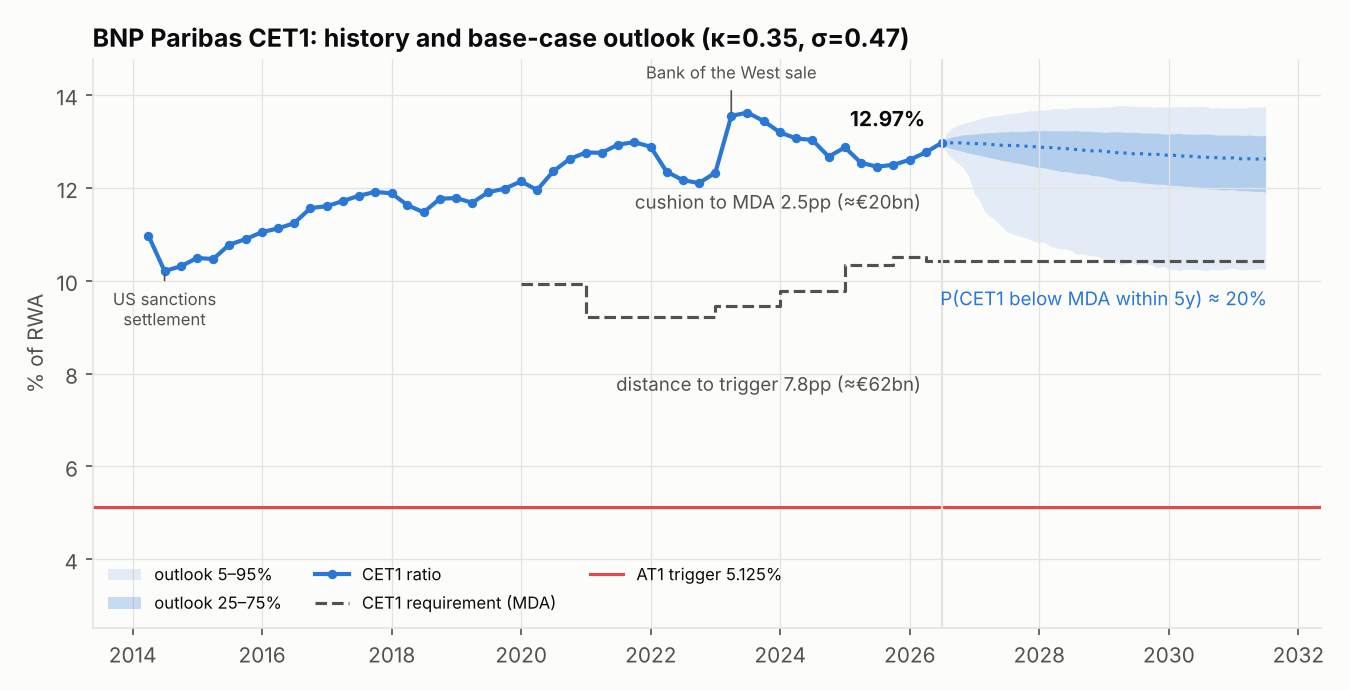
\includegraphics[width=0.85\textwidth]{bnp_cet1_history.png}
\caption{BNP Paribas CET1 ratio since 2014, CET1 requirement (MDA threshold), AT1 trigger
and the base-case five-year outlook (median, 50\% and 90\% bands of simulated CET1).}
\label{fig:cet1}
\end{figure}

\paragraph{Bootstrap.} To measure the precision of $\hat\kappa$ we simulate $1{,}000$
histories of the fitted process on the observed quarterly dates and re-estimate
$(\kappa,\sigma)$ on each. The $90\%$ intervals are $\kappa\in[0.063,\,0.476]$ and
$\sigma\in[0.37,\,0.52]$: the volatility is well identified, the speed of capital
rebuilding is not. The half-life of a capital shock lies between $1.5$ and $11$ years.
This is the familiar difficulty of estimating mean reversion from a short sample of a
persistent series, and it matters: Section~\ref{sec:uncert} shows that the capital stress
results scale by a factor of five across the interval.

\paragraph{Base case.} The base case uses $\kappa=0.35$ (half-life two years), inside the
bootstrap interval, with $\sigma=0.47$ re-estimated by \eqref{eq:sigmahat}. The
likelihood ratio statistic against the maximum likelihood estimate is $2\times1.5=3.0$,
below the $5\%$ critical value of $3.84$ for one restriction. Section~\ref{sec:uncert}
explains the choice: bond prices lean towards faster mean reversion, and BNP's explicit
capital management (a $13\%$ target with managed risk-weighted assets and distributions) is
consistent with it.

\paragraph{Jumps.} The jump parameters cannot be identified from fifty quarters with few
large shocks. We use $\lambda_J=0.12$ a year, $m_J=2.2$pp and $\sigma_J=0.5$. The $95$th
percentile of the jump size, $m_Je^{1.645\sigma_J-\sigma_J^2/2}=4.4$pp, matches the $4.2$pp
CET1 depletion of BNP in the EBA 2025 adverse scenario: the calibration says that a shock of
the size of the adverse scenario occurs as a single jump with probability
$0.12\times5\%=0.6\%$ a year, about once every 170 years; smaller jumps are more frequent and
can accumulate.

\subsection{Spread process and regulatory geometry}

The market component of the refinancing spread starts on each date at the average, across
the AT1s quoted that day, of the yield to first call minus the call-matched Treasury. It
mean-reverts at $a=0.5$ (half-life $1.4$ years) to the sample mean $\bar s=275$bp, with
volatility $\eta=100$bp and correlation $\rho=-0.3$ with capital shocks. The capital premium
is $\beta=1\%$ of spread per point of CET1 inside the buffer. Neither $\eta$ nor $\beta$
is identified by the data; Section~\ref{sec:results} reports the sensitivity of the
cross-section to $\eta$, and $\beta$ is discussed in Section~\ref{sec:discussion}. The MDA
geometry is as in \eqref{eq:mdathreshold}, the trigger is $5.125\%$, and the stressed share
price at conversion is $\xi=20\%$ of today's.

\subsection{Implied hazards and the cross-sectional test}

On each date and for each AT1 $j$ we solve $V^{(j)}_0(\lambda_j)=P_j^{\mathrm{clean}}+\mathrm{AI}_j$.
The three bonds share issuer, capital and trigger, so a correctly specified model should
give $\lambda_1=\lambda_2=\lambda_3$, and the dispersion
\[
  D=\max_j\lambda_j-\min_j\lambda_j
\]
is a specification test. It can also be used to ask which values of the unidentified
parameters ($\eta$, $\kappa$) the three prices are consistent with.

\paragraph{Power of the test.} The test has limited power with evaluated prices. By
Proposition~\ref{prop:shape}, a difference $\Delta\lambda$ in hazard corresponds to a price
difference of $|V_0'|\Delta\lambda$, with $|V_0'|=0.077$--$0.084$ points per basis point. The
bid--offer of $0.15$--$0.29$ points therefore corresponds to $1.9$--$3.5$bp of hazard. A
dispersion of a few basis points is within the precision of the data, and the test can
reject specifications that produce large dispersions but cannot rank specifications whose
dispersions differ by one or two basis points. Monte Carlo error is not the binding
constraint: the standard error of each implied hazard is $0.67$bp, and the dispersion,
computed on common random numbers, is more precise still.

\subsection{Tier~2 calibration and the identification of recovery}

On each date the Tier~2 and SNP notes are priced on the same simulated state as the AT1s,
with the spread process started at the same AT1 spread and the same CET1 print, and with
recoveries $R_{\mathrm{T2}}=20\%$ and $R_{\mathrm{SNP}}=40\%$, the Markit conventions for
subordinated and senior debt. Each bond gives an implied resolution hazard by
Proposition~\ref{prop:t2}; the Tier~2 2035NC34 is the anchor for $\lres$.

Recovery and hazard are not separately identified from a single bond: a higher recovery
requires a higher hazard to match the same price. With two bonds of the same tenor and
different seniority, Tier~2 and SNP, the restriction that both face the same resolution
hazard identifies one recovery given the other. We report the Tier~2 recovery $R^\star$
that equalises the two implied hazards given $R_{\mathrm{SNP}}=40\%$, and the sensitivity of
the AT1 split to $R_{\mathrm{T2}}$.
